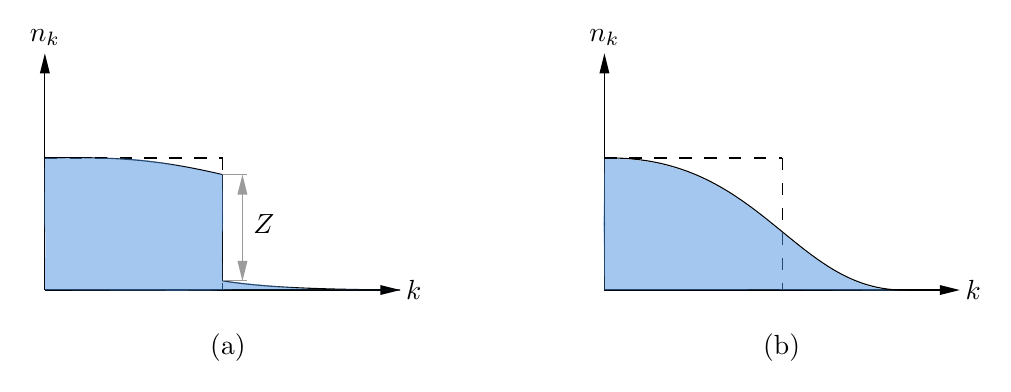
\begin{tikzpicture}[x=0.75pt,y=0.75pt,yscale=-0.8,xscale=0.8]
    %uncomment if require: \path (0,300); %set diagram left start at 0, and has height of 300
    
    %Straight Lines [id:da009219527738367317] 
    \draw    (405,225) -- (617,225) ;
    \draw [shift={(619,225)}, rotate = 180] [fill={rgb, 255:red, 0; green, 0; blue, 0 }  ][line width=0.08]  [draw opacity=0] (12,-3) -- (0,0) -- (12,3) -- cycle    ;
    %Straight Lines [id:da2079961540240256] 
    \draw    (405,225) -- (405,84.5) ;
    \draw [shift={(405,82.5)}, rotate = 90] [fill={rgb, 255:red, 0; green, 0; blue, 0 }  ][line width=0.08]  [draw opacity=0] (12,-3) -- (0,0) -- (12,3) -- cycle    ;
    %Straight Lines [id:da25299815998590813] 
    \draw  [dash pattern={on 4.5pt off 4.5pt}]  (405,145.5) -- (512,145.5) ;
    %Straight Lines [id:da23611716817469208] 
    \draw  [dash pattern={on 4.5pt off 4.5pt}]  (512,145.5) -- (512,224.5) ;
    %Curve Lines [id:da9173257888464759] 
    \draw    (405,145.5) .. controls (500,143.5) and (519,226.5) .. (587,225) ;
    %Curve Lines [id:da006174472132643993] 
    \draw [draw opacity=0][fill={rgb, 255:red, 74; green, 144; blue, 226 }  ,fill opacity=0.5 ]   (405,146) .. controls (500,144) and (519,227) .. (587,225.5) .. controls (404,224) and (589,225) .. (405,225) .. controls (404,147) and (404,223) .. (405,146) -- cycle ;
    %Straight Lines [id:da4367238433084937] 
    \draw    (68,225) -- (280,225) ;
    \draw [shift={(282,225)}, rotate = 180] [fill={rgb, 255:red, 0; green, 0; blue, 0 }  ][line width=0.08]  [draw opacity=0] (12,-3) -- (0,0) -- (12,3) -- cycle    ;
    %Straight Lines [id:da3594146199392185] 
    \draw    (68,225) -- (68,84.5) ;
    \draw [shift={(68,82.5)}, rotate = 90] [fill={rgb, 255:red, 0; green, 0; blue, 0 }  ][line width=0.08]  [draw opacity=0] (12,-3) -- (0,0) -- (12,3) -- cycle    ;
    %Straight Lines [id:da3068774329734081] 
    \draw  [dash pattern={on 4.5pt off 4.5pt}]  (68,145.5) -- (175,145.5) ;
    %Straight Lines [id:da14782967759901622] 
    \draw  [dash pattern={on 4.5pt off 4.5pt}]  (175,145.5) -- (175,224.5) ;
    %Curve Lines [id:da7552878456427861] 
    \draw    (68,145.5) .. controls (110,144.5) and (137,146.5) .. (175,155.5) ;
    %Curve Lines [id:da40499842494527183] 
    \draw    (175,219.5) .. controls (195,222.5) and (217,224.5) .. (282,225) ;
    %Straight Lines [id:da31095032234024567] 
    \draw    (175,155.5) -- (175,219.5) ;
    %Curve Lines [id:da9323659415170968] 
    \draw [draw opacity=0][fill={rgb, 255:red, 74; green, 144; blue, 226 }  ,fill opacity=0.5 ]   (68,145.5) .. controls (131,145.5) and (120,144.5) .. (175,155.5) .. controls (176,220.5) and (174,159.5) .. (175,219.5) .. controls (227,224.5) and (229,225.5) .. (282,225) .. controls (83,223.5) and (262,226.5) .. (68,225) .. controls (69,151.5) and (67,226.5) .. (68,145.5) -- cycle ;
    %Straight Lines [id:da2726570766053802] 
    \draw [color={rgb, 255:red, 155; green, 155; blue, 155 }  ,draw opacity=1 ]   (175,155.5) -- (190,155.5) ;
    %Straight Lines [id:da794346269199613] 
    \draw [color={rgb, 255:red, 155; green, 155; blue, 155 }  ,draw opacity=1 ]   (175,219.5) -- (190,219.5) ;
    %Straight Lines [id:da8221957579922665] 
    \draw [color={rgb, 255:red, 155; green, 155; blue, 155 }  ,draw opacity=1 ]   (187,157.5) -- (187,217.5) ;
    \draw [shift={(187,219.5)}, rotate = 270] [fill={rgb, 255:red, 155; green, 155; blue, 155 }  ,fill opacity=1 ][line width=0.08]  [draw opacity=0] (12,-3) -- (0,0) -- (12,3) -- cycle    ;
    \draw [shift={(187,155.5)}, rotate = 90] [fill={rgb, 255:red, 155; green, 155; blue, 155 }  ,fill opacity=1 ][line width=0.08]  [draw opacity=0] (12,-3) -- (0,0) -- (12,3) -- cycle    ;
    
    % Text Node
    \draw (621,225) node [anchor=west] [inner sep=0.75pt]    {$k$};
    % Text Node
    \draw (405,79.5) node [anchor=south] [inner sep=0.75pt]    {$n_{k}$};
    % Text Node
    \draw (284,225) node [anchor=west] [inner sep=0.75pt]    {$k$};
    % Text Node
    \draw (68,79.5) node [anchor=south] [inner sep=0.75pt]    {$n_{k}$};
    % Text Node
    \draw (192,178) node [anchor=north west][inner sep=0.75pt]    {$Z$};
    % Text Node
    \draw (166,250) node [anchor=north west][inner sep=0.75pt]   [align=left] {(a)};
    % Text Node
    \draw (499,250) node [anchor=north west][inner sep=0.75pt]   [align=left] {(b)};
    
    
\end{tikzpicture}
    